\documentclass[journal=jacsat,manuscript=article]{achemso}
\usepackage[latin1]{inputenc}
\usepackage{amsmath}
\usepackage{amsfonts}
\usepackage{amssymb}
\usepackage{graphicx}
\usepackage{numprint}
\usepackage{mathtools}
\usepackage{enumitem}
\usepackage{hyperref}
\usepackage[squaren,grey]{SIunits}
\usepackage{setspace}
\doublespacing

\author{Haina Wang}
\affiliation[Princeton University]{Department of Chemistry Torquato Lab, Princeton University, Princeton, NJ 08544, USA}
\email{hainaw@princeton.edu}

\title{Structure factors}
  
\begin{document}
	\maketitle

	\newpage
	\section{Analytical structure factor of 1D lattice}
	The length of the cell $L=1$. The number of particles $N = 2,3,...,10$.
	
	\begin{figure}
		\includegraphics[width=1\linewidth]{sk1d}
		\caption{The analytical $S(k)$ of 1D lattice.}
		\label{fig:sk1d}
	\end{figure}

	\newpage
	\section{Equilibrium 3D hard spheres}
	\begin{figure}
		\centering
		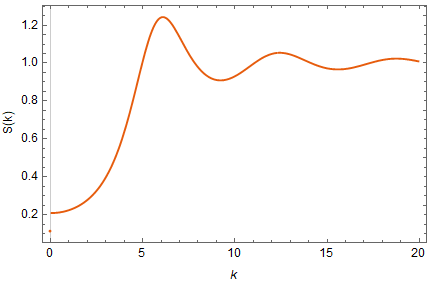
\includegraphics[width=0.7\linewidth]{C:/Users/Nora/Documents/G1.5/StrucFac/theoreticalPhi0_2}
		\caption{The theoretical $S(k)$ for equilibrium 3D hard spheres in the PY approximation with $\Phi = 0.2$.}
		\label{fig:theoreticalphi0}
	\end{figure}
	

\end{document}
